% =========================================================================
% KSTAR CES multimodal nowcasting — conference-style draft
% Build: pdflatex main && bibtex main && pdflatex main && pdflatex main
% NOTE: written against the generic article class so it compiles anywhere;
% swap the preamble for a specific conference template (NeurIPS/ICML/IAEA)
% without touching the body.
% =========================================================================
\documentclass[10pt]{article}

\usepackage[margin=1in]{geometry}
\usepackage[T1]{fontenc}
\usepackage[utf8]{inputenc}
\usepackage{amsmath,amssymb,bm}
\usepackage{graphicx}
\usepackage{booktabs}
\usepackage{multirow}
\usepackage{microtype}
\usepackage[numbers,sort&compress]{natbib}
\usepackage[colorlinks=true,linkcolor=blue,citecolor=blue,urlcolor=blue]{hyperref}
\usepackage{xcolor}

\newcommand{\todo}[1]{\textcolor{red}{[TODO: #1]}}
\newcommand{\Ti}{\ensuremath{T_i}}
\newcommand{\Vrot}{\ensuremath{V_\mathrm{rot}}}
\newcommand{\skillp}{\ensuremath{\mathrm{skill}_{\mathrm{PCHIP}}}}

\graphicspath{{figures/}}

\title{\textbf{Multimodal Nowcasting of Sparse Charge-Exchange Spectroscopy on KSTAR:\\
Fast Diagnostics Recover Ion Temperature Beyond Future-Using Interpolation,\\
but Not Toroidal Rotation}}

\author{%
  Seungsang Lee\\
  Department of Nuclear Engineering, Seoul National University\\
  \texttt{lss010330@snu.ac.kr}
}

\date{Draft --- \today}

\begin{document}
\maketitle

% =========================================================================
\begin{abstract}
Charge-exchange spectroscopy (CES) is the primary measurement of ion temperature
(\Ti) and toroidal rotation (\Vrot) in tokamaks, but photon-collection constraints
make it slow and intermittently missing: on the KSTAR 10\,ms grid studied here,
$\approx$8\% of \Ti{} and $\approx$24\% of \Vrot{} samples are absent, and the two
targets go missing independently. We ask whether the always-available fast
diagnostics---beam-emission spectroscopy (BES), electron-cyclotron-emission imaging
(ECEI), and Mirnov coils---together with the irregular past CES history can recover
information at missing CES timesteps that \emph{temporal interpolation of CES alone
cannot}. We train a compact ($<$1M-parameter) multimodal network with per-diagnostic
encoders, explicit irregular-time features, per-target masked losses, and
physics-informed per-target input routing, and evaluate it against a deliberately
adverse bar: offline interpolation (linear, monotone-cubic PCHIP, local AR) that is
allowed to see \emph{past and future} CES neighbors, while the model is strictly
causal. Under a pre-registered protocol---file-level train/val/test splits, a test
set never touched by model selection, and a shot-clustered paired bootstrap
(10{,}000 resamples)---the model beats PCHIP on \Ti{} with skill $+0.20$ to $+0.30$
and a 95\% CI excluding zero on \emph{four independent held-out splits}, while
\Vrot{} is statistically indistinguishable from interpolation on all four. Input
ablations show this asymmetry is physical rather than architectural: fast
diagnostics alone beat persistence for \Ti{} (collisional $e$--$i$ coupling makes
$T_e$ and $n_e$ informative) but are far worse than the mean for \Vrot{} (the
dominant NBI torque is unobserved and 100\,Hz-sampled Mirnov signals alias away kHz
mode rotation). The model's advantage concentrates in high-local-variability
neighborhoods where smooth interpolation is weakest. We also document a
data-quality audit (54\% of observed \Vrot{} values are forward-filled instrument
holds) and an LLM-driven keep/discard architecture-search loop that turned an
initially non-significant result into the significant headline. We release the
full pipeline, pre-registration, and evaluation artifacts.
\end{abstract}

% =========================================================================
\section{Introduction}
\label{sec:intro}

Ion temperature \Ti{} and toroidal rotation \Vrot{} at the plasma edge govern key
elements of tokamak performance and stability, including pedestal structure, ELM
behavior, and access to high-confinement regimes. The workhorse measurement of both
quantities is charge-exchange spectroscopy (CES)~\citep{Ko2010ChargeExchange},
which infers \Ti{} from Doppler broadening and \Vrot{} from the
Doppler shift of charge-exchange line emission. Because CES must integrate photons
to reach adequate signal-to-noise, it is intrinsically slow, and individual time
points are frequently lost to exposure and signal-quality problems. In the KSTAR
data studied here, even on a uniform 10\,ms grid, $\approx$8\% of \Ti{} and
$\approx$24\% of \Vrot{} observations are missing---\emph{independently} of each
other---and, empirically in our dataset, the missingness concentrates at
physically interesting moments (low signal-to-noise phases, ELMs, transitions),
i.e.\ it is missing-not-at-random in the sense of
\citet{Little2002StatisticalAnalysis} (MNAR).

Meanwhile, several fast diagnostics observe the same plasma without gaps: BES
measures density-fluctuation structure, ECEI images electron temperature, and
Mirnov coils record magnetic fluctuations. None of them measures \Ti{} or \Vrot{}
directly. The question this paper asks is:

\begin{quote}
\emph{At a 10\,ms timestep where CES is missing, can the simultaneous fast
diagnostics plus the irregular past CES history recover \Ti{} and \Vrot{}
information that temporal interpolation of CES alone cannot?}
\end{quote}

A positive answer would justify a data-driven \emph{virtual sensor}: a model that
fills CES gaps online, without the strong inverse-mapping assumptions required by
hardware alternatives, enabling gap-free pedestal analysis and, ultimately,
real-time use.

\paragraph{A deliberately hard bar.}
The obvious baseline for gap-filling is interpolation of the CES channel itself.
We make the comparison intentionally adverse to the model: the interpolation
baselines (linear, monotone-cubic PCHIP~\citep{fritsch1980}, and a local AR
reference) are \emph{offline}---they may use CES neighbors on \emph{both sides} of
the target time, including the future---whereas the model is strictly causal,
seeing only the fast diagnostics at the target step and a short window of past CES.
If a causal model beats a future-using interpolant, the fast diagnostics must carry
CES-relevant information that the temporal structure of CES alone does not contain;
and a model that beats future-using interpolation a fortiori beats every causal
baseline (persistence, AR).

\paragraph{Contributions.}
\begin{enumerate}
  \item \textbf{A leakage-hardened multimodal nowcasting pipeline} for sparse,
        irregularly observed CES targets: per-target masked multitask losses that
        recover the $\approx$28\% of labeled rows discarded by both-targets-required
        filtering; explicit irregular-time features; full masking of the target
        timestep in the CES-history input; file-level (shot-level) splits; and
        train-file-only normalization statistics (\S\ref{sec:data}).
  \item \textbf{A pre-registered, shot-clustered evaluation protocol}
        (\S\ref{sec:eval}) with a three-way split whose test set is never read by
        model selection, and significance assessed by a shot-clustered paired
        bootstrap---adjacent samples within a discharge are strongly correlated, so
        the discharge, not the sample, is the unit of replication.
  \item \textbf{A robust positive result for \Ti{}} (\S\ref{sec:results}): the
        causal model beats future-using PCHIP interpolation with
        $\skillp = +0.20$ to $+0.30$ and shot-clustered 95\% CIs excluding zero on
        four independent held-out splits, and survives a genuine-measurement-only
        re-evaluation.
  \item \textbf{A physics-grounded negative result for \Vrot{}}, reported as a
        finding rather than a failure: fast diagnostics carry essentially no
        rotation information at 10\,ms (unobserved NBI torque; Mirnov aliasing),
        confirmed by input ablations, so \Vrot{} remains
        history-autocorrelation-limited and statistically ties interpolation. We
        call this the \Ti$\leftrightarrow$\Vrot{} \emph{information asymmetry}.
  \item \textbf{Diagnosis of where the model earns its edge}: skill is concentrated
        in high-local-variability neighborhoods, where smooth interpolation is
        weakest; there, even \Vrot{} shows a (fragile) significant edge, and an
        ablation shows the \Ti{} edge genuinely uses the multimodal signal.
  \item \textbf{Two methodological artifacts}: a data-quality audit revealing that
        54\% of observed \Vrot{} values are forward-filled instrument holds (and a
        corrected evaluation), and an LLM-driven keep/discard architecture-search
        loop whose selection gate is the clean interpolation-relative skill rather
        than validation loss.
\end{enumerate}

% =========================================================================
\section{Related work}
\label{sec:related}

\paragraph{Profile fitting and gap-filling in fusion diagnostics.}
Gaussian-process regression~\citep{rasmussen2006} is the community-standard tool
for fitting and uncertainty-quantifying fusion profile
data~\citep{chilenski2015,michoski2024}, and monotone interpolants such as
PCHIP~\citep{fritsch1980,dougherty1989} are preferred over natural cubic
splines~\citep{reinsch1967} near transients because splines exhibit Gibbs-like
ringing at ELM- and sawtooth-like steps~\citep{kvernadze1998}. Irregularly
sampled series admit exact AR-type null models
(IAR/CIAR)~\citep{eyheramendy2018,elorrieta2019}. We use this
ladder---persistence, linear interpolation~\citep{press2007}, PCHIP, local
AR---as pre-registered baselines, with PCHIP as
the headline comparator, and Murphy's MSE skill score~\citep{murphy1988} as the
metric. Our contribution is orthogonal to this literature: rather than a better
CES-only interpolant, we test whether \emph{other diagnostics} add information
beyond any CES-only method, by benchmarking a causal multimodal model against
future-using interpolation.

\paragraph{Neural diagnostic inference in fusion.}
Neural diagnostic inference has three main lines, and it is instructive to ask
of each: \emph{what happens when the target measurement is absent?} The oldest
line accelerates spectral fitting---NN analysis of JET CX
spectra~\citep{Bishop1993AutomaticAnalysis,Svensson1999AnalysisJet} and fast
\Ti{} estimation from EAST CXRS spectra~\citep{Chai2019FastEstimation}. These
gain orders of magnitude in speed over least-squares fits, but by construction
they require measured spectra at the timestep: a missing CES exposure leaves
them with no input at all. A second line replaces one inference pipeline with
another diagnostic's: Bayesian-model emulation at
W7-X~\citep{Pavone2019NeuralNetwork}, profile shapes from scalar parameters on
NSTX-U~\citep{Boyer2021PredictionElectron}, and---closest to our targets---\Ti{}
and rotation profiles from an x-ray crystal spectrometer on
EAST~\citep{Lin2024PredictionPlasma}. Lin et al.\ predict exactly our two
quantities, but from another Doppler spectrometer, i.e.\ the same physical
information channel with the same photon-statistics limits; the mapping is
instantaneous and inherits the source diagnostic's availability. A third line
builds end-to-end surrogates for slow reconstruction codes: bolometer
tomography~\citep{Matos2016DeepLearning}, line-integral
diagnostics~\citep{Wang2025PhysicsinformedDeep}, safety-factor
profiles~\citep{Wei2023ReconstructionTokamak}, real-time
equilibria~\citep{Zheng2024RealtimeEquilibrium}, and---on KSTAR itself---NN
Grad--Shafranov solvers~\citep{Joung2020DeepNeural,Joung2023GsdeepnetMastering}
and rapid EPED-parameterized profile
reconstruction~\citep{Jung2026MachineLearningbased}. These address analysis
\emph{latency}, not measurement \emph{availability}: they accelerate inversions
of data that exist. Two works sit closer to the availability question.
Actuator-conditioned profile forecasting on
DIII-D~\citep{Abbate2021DatadrivenProfile} is causal and history-driven like our
model, but forecasts from \emph{dense} measured profiles for control, rather
than recovering a sparse channel. RTCAKENN~\citep{Shousha2023MachineLearningbased}
reconstructs kinetic profiles (including impurity temperature and rotation) in
real time and keeps operating when Thomson/CER inputs drop out, via dropout
training; missingness there is a robustness condition handled by zeroing inputs,
whereas in our setting the target's own sparsity is the problem itself, tracked
explicitly through per-target observation flags and irregular-time features.
Across all three lines the common assumption is that the information source is
available when the model runs; recovering a diagnostic at timesteps where
\emph{its own} measurement is missing, from other channels plus its past, falls
outside their scope.

\paragraph{Cross-diagnostic reconstruction and temporal densification (closest prior work).}
A recent family reconstructs one diagnostic from others. GP-based imputation
restores faulty magnetic sensors on KSTAR in
sub-ms~\citep{Joung2018ImputationFaulty}; ML detects and compensates corrupted
sensors~\citep{Mohapatra2019RealtimeSensor}; autoencoders fuse redundant density
diagnostics for resilience~\citep{Kaldas2026DevelopingAutoencoder}; time-series
extrinsic regression fills missing electron-temperature data on
EAST~\citep{Wang2025TimeSeries}; and FusionMAE performs masked-channel ``virtual
backup diagnosis'' across 88 channels on HL-3~\citep{Yang2026FusionmaeSelfsupervised}.
Closest to our framing, Diag2Diag synthesizes Thomson-scattering $T_e$/$n_e$ at
fluctuation-diagnostic rates from other simultaneous diagnostics on
DIII-D~\citep{Jalalvand2025MultimodalSuperresolution}, and temporal
super-resolution of Thomson profiles from fast radiation diagnostics has been
demonstrated on COMPASS~\citep{Imrek2026TemporalSuperresolution}; PanoMHD models
multimodal signal dynamics with a causal transformer for
control~\citep{Noh2026PanomhdMultimodal}. Our work differs from this family on
four axes, each verifiable from the cited works' stated scope: (i) \emph{target
channel}---every member reconstructs electron quantities or generic dense
channels (Thomson $T_e$/$n_e$ in \citealp{Jalalvand2025MultimodalSuperresolution}
and \citealp{Imrek2026TemporalSuperresolution}; ECE-type $T_e$ in
\citealp{Wang2025TimeSeries}; arbitrary masked channels in
\citealp{Yang2026FusionmaeSelfsupervised}), and where CER/CES appears at all it
is an \emph{input}~\citep{Jalalvand2025MultimodalSuperresolution}, never the
sparse target; (ii) \emph{causality}---Diag2Diag and the COMPASS study are
simultaneous, memory-less mappings, and FusionMAE reconstructs within a window,
whereas our model conditions on the target's own irregular past and never reads
the future; (iii) \emph{evaluation bar}---none benchmarks against
\emph{future-using} interpolation of the target channel, which for gap-filling
is the incumbent method to beat, under a pre-registered shot-clustered protocol;
and (iv) \emph{information analysis}---reconstructability is assumed rather than
tested per target, whereas the \Ti$\leftrightarrow$\Vrot{} asymmetry is our
central finding. Within the surveyed literature we found no causal temporal
gap-filling of sparse CXRS ion measurements on any device; we state this as the
outcome of our literature search, not as a claim that no such attempt exists.

\paragraph{Irregular-time and masked multitask learning.}
Our design borrows standard ingredients from the irregular time-series
literature---observation masks and decay-aware recurrence
(GRU-D~\citep{Che2018RecurrentNeural}), attention over continuous-time
embeddings (mTAN~\citep{Shukla2021MultitimeAttention}), and latent-ODE
dynamics~\citep{Rubanova2019LatentOrdinary}---together with multitask learning
under partial labels~\citep{Caruana1997MultitaskLearning}, late-fusion multimodal
architectures~\citep{Ngiam2011MultimodalDeep,Baltruaitis2018MultimodalMachine},
pre-LayerNorm transformers~\citep{Xiong2020LayerNormalization}, and attention
pooling~\citep{Ilse2018AttentionbasedDeep}. The ``nowcasting'' framing follows
its use in machine-learning weather
prediction~\citep{Shi2015ConvolutionalLstm,Ravuri2021SkilfulPrecipitation}. The
novelty is not any single ingredient but the leakage-hardened combination under a
physics-adverse evaluation protocol.

% =========================================================================
\section{Data and problem setup}
\label{sec:data}

\subsection{Dataset}
We use 641 KSTAR discharge (shot) files, prioritized from campaigns
\#24000--\#33000 for hardware consistency, targeting H-mode ELM-suppression (RMP)
phases; segments of $\sim$100\,ms are cut around D$_\alpha$-active intervals. All
signals are aligned to a common 10\,ms grid. Each row provides
BES~\citep{Nam2012AnalysisEdge} (9 channels), ECEI~\citep{Yun2010DevelopmentKstar}
(4 channels), Mirnov coils (2 channels), time, and the two CES targets
\Ti{} and \Vrot{}~\citep{Ko2010ChargeExchange}. On this grid \Ti{} is missing in $\approx$8\% of rows and
\Vrot{} in $\approx$24\%, independently (Fig.~\ref{fig:missing}).

\begin{figure}[t]
  \centering
  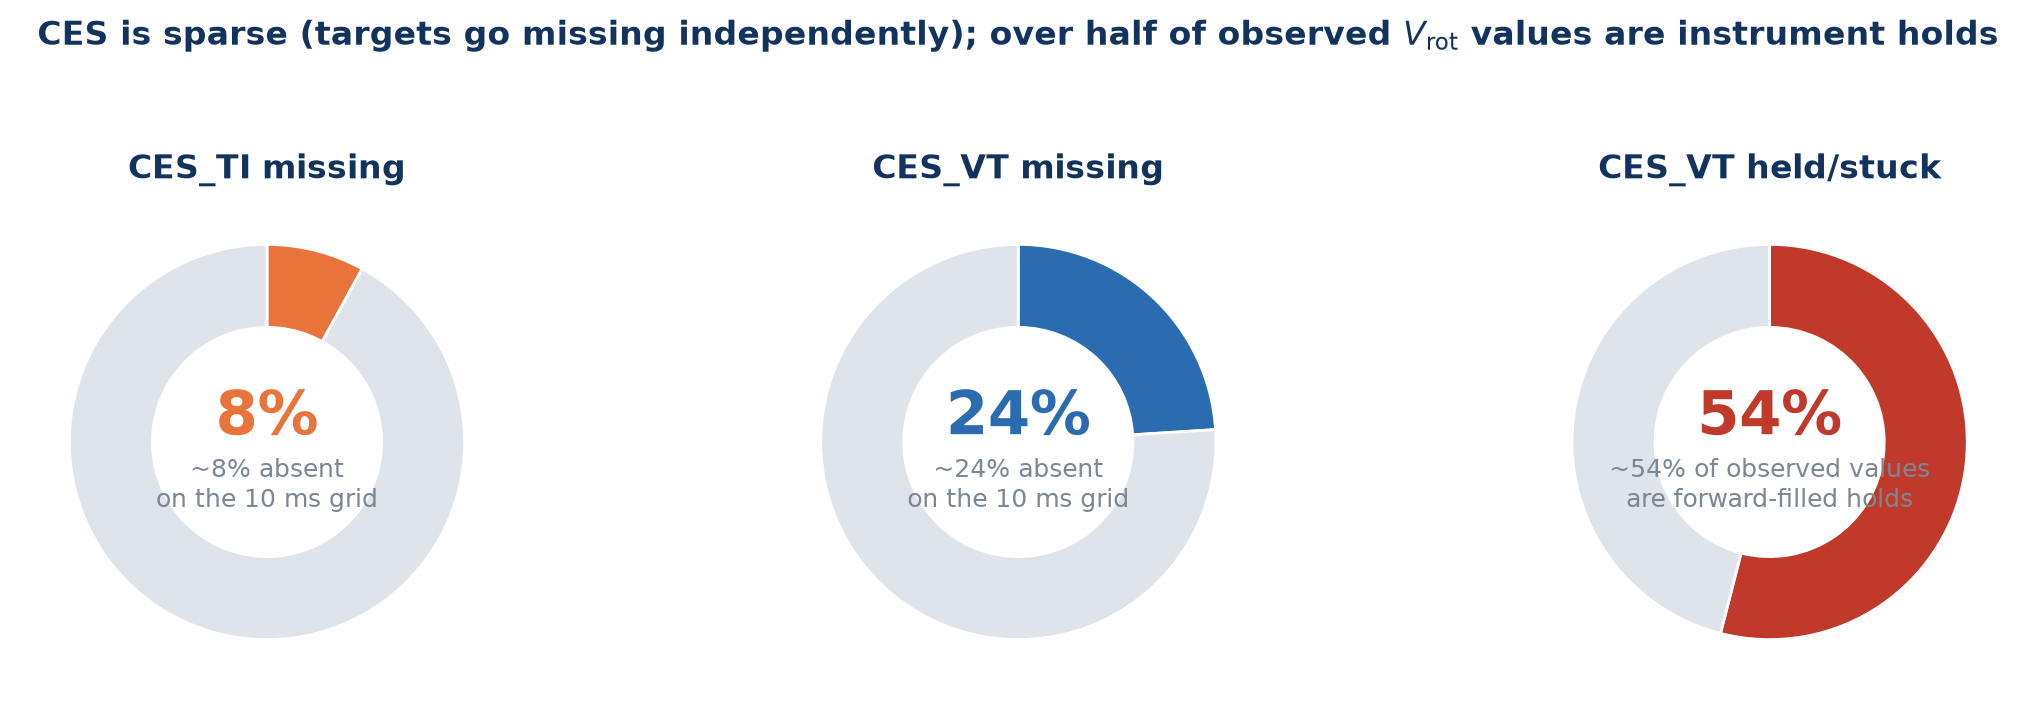
\includegraphics[width=0.72\linewidth]{fig_missing}
  \caption{CES missingness structure on the 10\,ms grid. \Ti{} and \Vrot{} go
  missing independently ($\approx$8\% / $\approx$24\%), motivating per-target
  masking rather than row filtering.}
  \label{fig:missing}
\end{figure}

\subsection{Sample construction}
A training sample at target index $t$ with history window $W{=}4$ consists of
\texttt{bes} $(W,9)$, \texttt{ecei} $(W,4)$, \texttt{mc} $(W,2)$,
\texttt{time\_features} $(W,4)$, \texttt{ces\_history} $(W,4)$, the normalized
target $[\Ti,\Vrot]\in\mathbb{R}^2$, and a per-target observation mask
$m\in\{0,1\}^2$. The four time features---lookback seconds, inter-row delta
seconds, and their $\log(1{+}x)$ transforms---expose the irregular observation
pattern to the model explicitly: the reliability of a past CES value depends
strongly on whether it is 10\,ms or 200\,ms old. The four CES-history channels are
the previous normalized \Ti{}, previous normalized \Vrot{}, and one observation
flag per target (the targets go missing independently, so observation must be
tracked per target).

\subsection{Design principles}
\begin{description}
  \item[No fabricated labels.] We never impute targets to create training rows. A
  row is kept iff its diagnostic inputs are complete and \emph{at least one} CES
  target is genuinely observed.
  \item[Per-target masked loss.] The loss is masked per target,
  $\mathcal{L} = \sum_{k\in\{\Ti,\Vrot\}} m_k\,(\hat{y}_k-y_k)^2 / \sum_k m_k$,
  so a row with only one observed target still supervises that target. The
  previous both-targets-required filter silently discarded $\approx$28\% of
  labeled rows; removing it is a pure data gain.
  \item[Leakage hardening.] (i) \emph{File-level splits}: adjacent rows within a
  shot are strongly autocorrelated, so splits are made at the shot-file level and
  pinned to disk; (ii) \emph{train-file-only normalization}: all $z$-score
  statistics (NaN-aware for the sparse targets) are estimated on training files
  only; (iii) \emph{target-step masking}: in \texttt{ces\_history}, the target
  timestep's values \emph{and} observation flags are zeroed, so the model cannot
  read its own answer.
\end{description}

\subsection{Data-quality audit: held (forward-filled) \Vrot{} values}
\label{sec:stuck}
A late audit found that \textbf{54\% of observed \Vrot{} values are instrument
holds}: bit-identical repeats of the previous observation within a contiguous time
block (runs up to 1{,}214 rows; 499/641 files affected). These arise because the
native \Vrot{} cadence is slower than the row cadence; they are not independent
measurements. \Ti{} is unaffected (0.0\%). A controlled A/B retrain showed
training is \emph{not} contaminated---masking holds at train time does not improve
(and slightly hurts) genuine-measurement performance, i.e.\ the holds act as a
harmless persistence prior---so holds are kept in training but \emph{excluded from
evaluation}. The correction inflates reported physical \Vrot{} RMSE by
35--55\% (from 22--33 to 35--46 in raw units) because held targets have near-zero
baseline error; all conclusions below use the corrected (genuine-only) evaluation,
and the \Ti{} headline is unchanged by it.

% =========================================================================
\section{Model}
\label{sec:model}

The predictor is a compact ($<$1M parameters) late-fusion network; the bottleneck
in this problem is generalization, not capacity.

\paragraph{Per-diagnostic encoders.}
Each modality (BES, ECEI, MC) is encoded by its own time-aware 1-D CNN that
consumes the modality jointly with the time features and history, preserving each
diagnostic's channel structure until fusion. CNNs are preferred over recurrence
because gap-removal makes the effective sampling irregular, violating the
uniform-step assumption RNNs rely on.

\paragraph{History encoder.}
The CES history is encoded by a 2-layer pre-LayerNorm
Transformer~\citep{Xiong2020LayerNormalization} with learned positional
embeddings and \emph{multi-head attention
pooling}~\citep{Ilse2018AttentionbasedDeep} that outputs both an
attention-weighted mean and an attention-weighted standard deviation; the latter
exposes ``how locally variable is the recent history,'' which
\S\ref{sec:peak} shows is where the model earns its edge. Self-attention over the
(masked) target step and its observed neighbors performs an operation analogous to
learned interpolation, with per-target observed-neighbor biases.

\paragraph{Physics-informed per-target routing.}
The \Ti{} head fuses fast diagnostics + time + history; the \Vrot{} head fuses
\emph{history and time only}, deliberately excluding the fast diagnostics, which
ablations (\S\ref{sec:asym}) show carry no usable rotation information at 10\,ms.
Each target has its own pre-LayerNorm MLP head; outputs remain in normalized units
(denormalization happens only in evaluation).

\paragraph{Search lessons.}
Across $\sim$40 controlled architecture iterations, pre-LayerNorm was the
stability turning point (validation loss $0.89\!\to\!0.49$), attention pooling was
the most reliable single improvement, and aggressive capacity scaling, complex
skip topologies, and extra convolutional extractors consistently failed to improve
held-out performance.

% =========================================================================
\section{Evaluation methodology}
\label{sec:eval}

\paragraph{Metric.}
All errors are denormalized to physical CES units and computed per target. The
primary score is Murphy's skill~\citep{murphy1988} against the pre-registered
headline baseline,
$\skillp = 1 - \mathrm{MSE}_{\mathrm{model}}/\mathrm{MSE}_{\mathrm{PCHIP}}$
(positive = model better; 0 = tie). Every arm (model and all baselines) is scored
on the \emph{identical} (file, row) sample set under the same per-target keep
mask. Interpolants exclude the target's own value (no leakage) and refuse to
interpolate across gaps $\geq 0.5$\,s, falling back to persistence.

\paragraph{Three-way split; selection never sees TEST.}
Files are split train/val/test; the test set was reserved \emph{before} any
architecture search and is never read by the search loop, so headline numbers
carry no winner's-curse bias. The canonical test set contains 34{,}644 scored
samples across 96 shots (observed $n$: \Ti{} 32{,}716, \Vrot{} 27{,}437).

\paragraph{Pre-registration.}
Four rules were fixed in writing before viewing test numbers:
\textbf{PR1} the headline comparator is PCHIP (chosen a priori for
monotonicity/no ringing at transients; the full ladder
\{persistence, linear, PCHIP, AR\} is also reported);
\textbf{PR2} interpolation predicts everywhere the model is scored, with
persistence fallback where no future neighbor exists (no population thinning);
\textbf{PR3} a minimum test-set floor ($\geq$15 shots, $\geq$3{,}000 observed
\Ti{} samples; met);
\textbf{PR4} significance means a shot-clustered bootstrap 95\% CI on the skill
excluding zero.

\paragraph{Shot-clustered paired bootstrap.}
Adjacent CES rows within a discharge are strongly correlated; treating samples as
independent would grossly understate uncertainty. Per-sample paired errors
$\mathrm{SE}_{\mathrm{model}}-\mathrm{SE}_{\mathrm{PCHIP}}$ are aggregated by
shot, and whole shots are resampled with replacement (10{,}000 resamples, fixed
seed). The resulting CI reflects genuine shot-to-shot generalization; its cost is
that the effective sample size is the number of shots ($\approx$96), which bounds
statistical power throughout.

\paragraph{Honest caveat (MNAR).}
Truly missing points have no ground truth, so skill is measured by masking
\emph{observed} points. Because CES missingness is MNAR (drop-out at low S/N,
ELMs, transitions), observed-point skill is an \emph{optimistic bound} for
performance at genuinely missing points. We state this rather than hide it.

% =========================================================================
\section{Results}
\label{sec:results}

\subsection{The model dominates every causal baseline}
Table~\ref{tab:ladder} shows the physical-unit RMSE ladder on the canonical test
split. The model has the lowest RMSE for both targets and beats the causal
baselines---persistence and past-only AR, i.e.\ everything actually available in
real time---by a wide margin. This is the most robust result in the paper: for any
online setting, where future CES is by definition unavailable, the model is the
clear winner.

\begin{table}[t]
  \centering
  \caption{Physical-unit RMSE ladder on the canonical held-out test split
  (pre-improvement baseline model; the final model improves further, see
  \S\ref{sec:headline}). Lower is better. \Vrot{} RMSE values here predate the
  hold correction of \S\ref{sec:stuck}; corrected genuine-only \Vrot{} RMSE is
  35--46.}
  \label{tab:ladder}
  \small
  \begin{tabular}{llrr}
    \toprule
    Arm & Information access & \Ti{} RMSE & \Vrot{} RMSE \\
    \midrule
    \textbf{Model (nowcaster)} & fast diag.\ + past CES & \textbf{412.4} & \textbf{23.2} \\
    Linear interpolation & past + future CES & 422.7 & 24.0 \\
    PCHIP interpolation & past + future CES & 431.8 & 24.5 \\
    Persistence & last observed CES & 487.3 & 27.8 \\
    AR (local, causal) & past CES only & 1005.7 & 57.2 \\
    \bottomrule
  \end{tabular}
\end{table}

\begin{figure}[t]
  \centering
  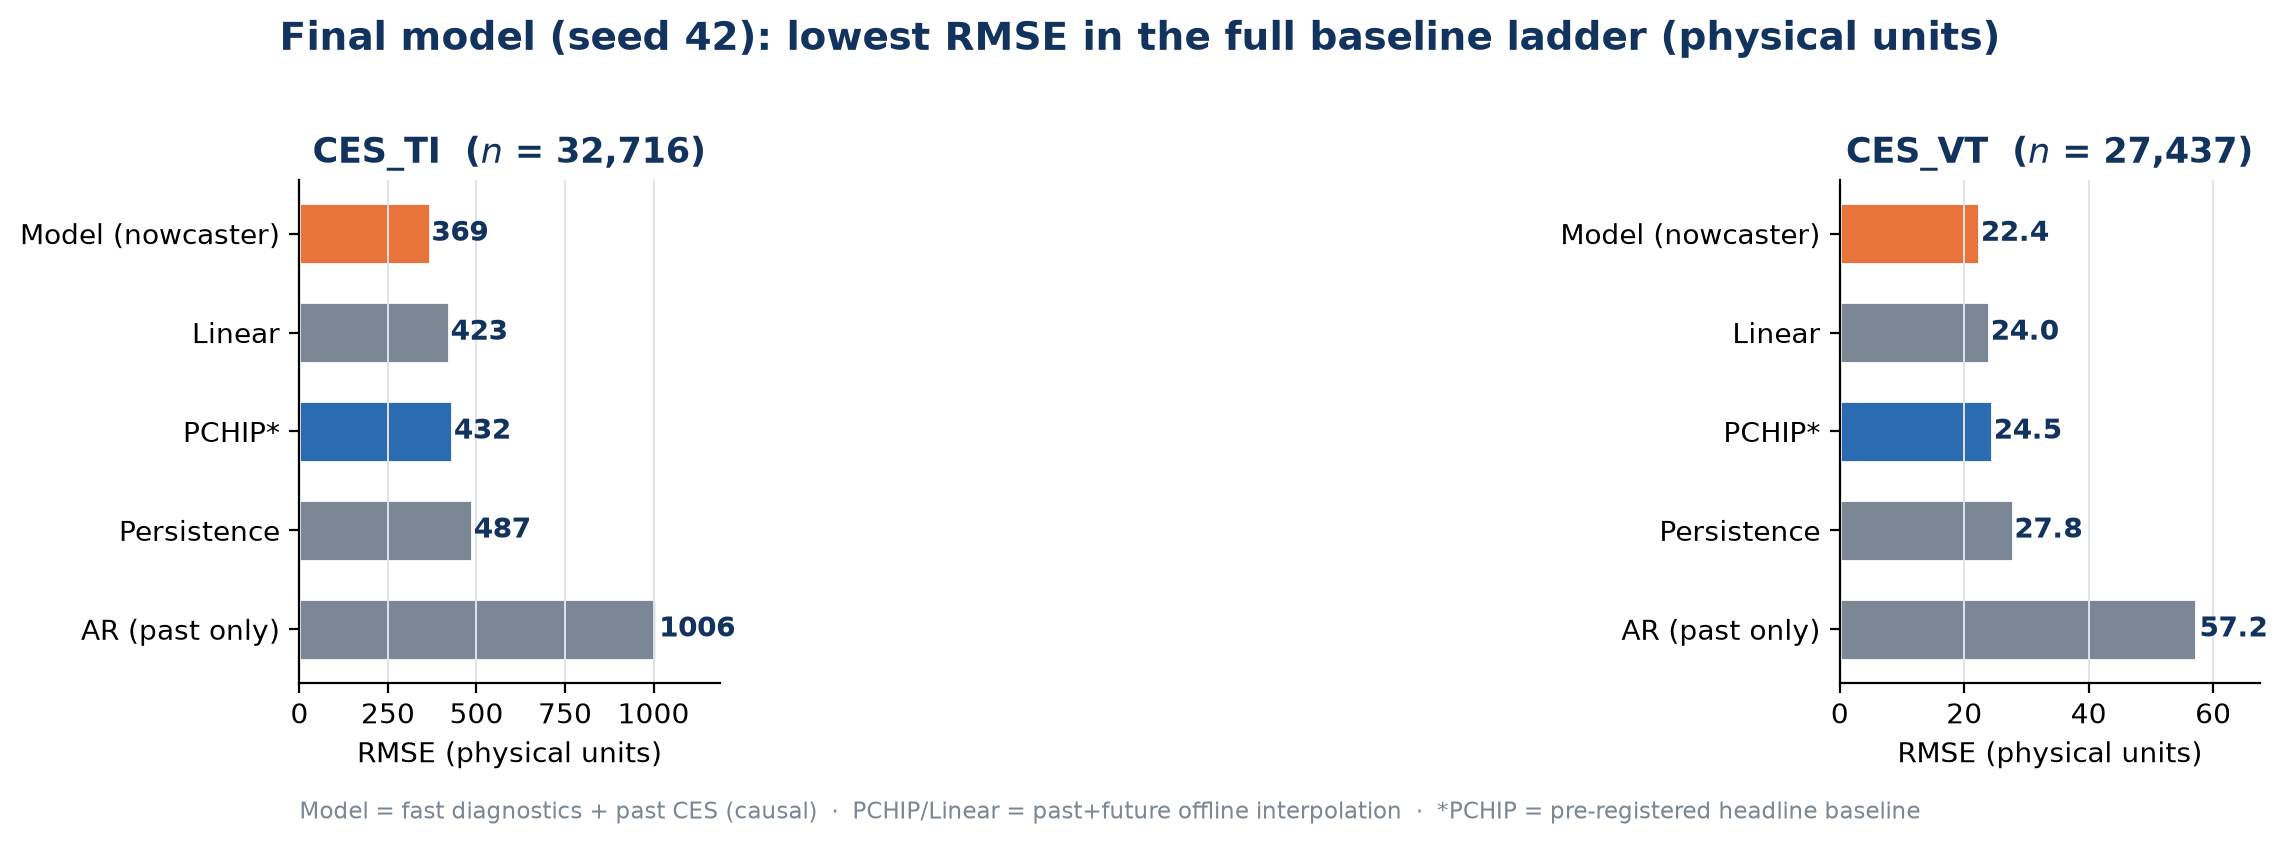
\includegraphics[width=0.8\linewidth]{fig_rmse_ladder}
  \caption{RMSE ladder for the \emph{final} model (seed 42, test split): the
  causal model attains the lowest RMSE for both targets, decisively beating the
  causal baselines and edging the future-using interpolants on the point
  estimate. Table~\ref{tab:ladder} reports the same ladder for the earlier
  baseline model, hence the different absolute values.}
  \label{fig:ladder}
\end{figure}

\subsection{Headline: \Ti{} beats future-using interpolation on four independent splits}
\label{sec:headline}
With the final architecture (GRU history encoder + per-target multi-head-attention
heads, $W{=}4$; selected by the search loop of \S\ref{sec:automl} on validation
skill only), we evaluated four \emph{independent} held-out test splits (seeds 42,
1, 7, 123; the latter three were never used in any selection step):

\begin{itemize}
  \item \textbf{\Ti{}: PASS on all four splits.}
        $\skillp = +0.270$ (95\% CI $[+0.144, +0.364]$), $+0.200$, $+0.271$,
        $+0.295$; every shot-clustered CI excludes zero, against both PCHIP and
        linear. The result survives genuine-measurement-only re-evaluation
        ($+0.225/+0.204/+0.285/+0.288$, all PASS).
  \item \textbf{\Vrot{}: not significant on any split.} Point estimates are
        positive but every CI includes zero. We claim a tie, not a win.
\end{itemize}

\begin{figure}[t]
  \centering
  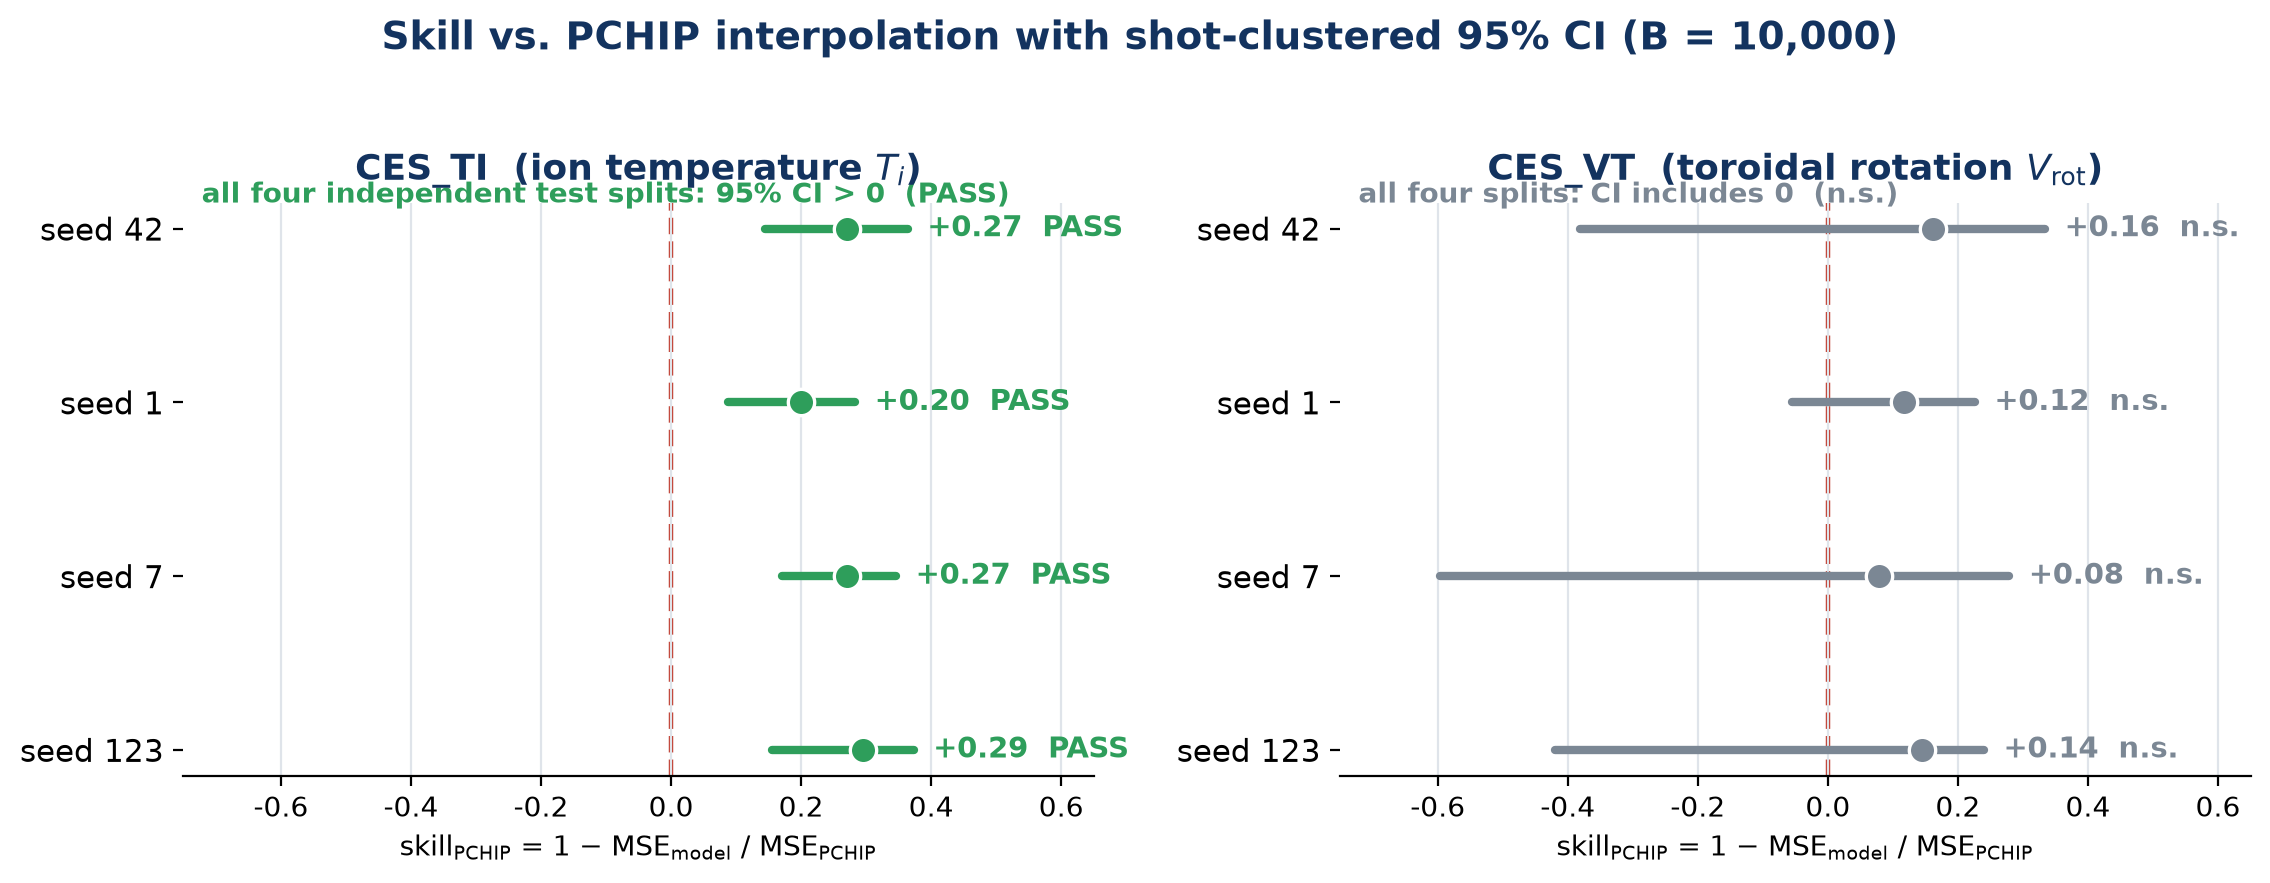
\includegraphics[width=0.78\linewidth]{fig_forest}
  \caption{Forest plot of $\skillp$ with shot-clustered 95\% CIs across four
  independent held-out splits. \Ti{} excludes zero on all four; \Vrot{} on none.}
  \label{fig:forest}
\end{figure}

An honest progression note: the initial baseline model was \emph{not} significant
(single split, $+0.088$, n.s.). Switching the architecture-search selection gate
from validation loss to the clean interpolation-relative skill produced the final
model, which is significant on all four splits (Fig.~\ref{fig:progression}). We
report both stages.

\begin{figure}[t]
  \centering
  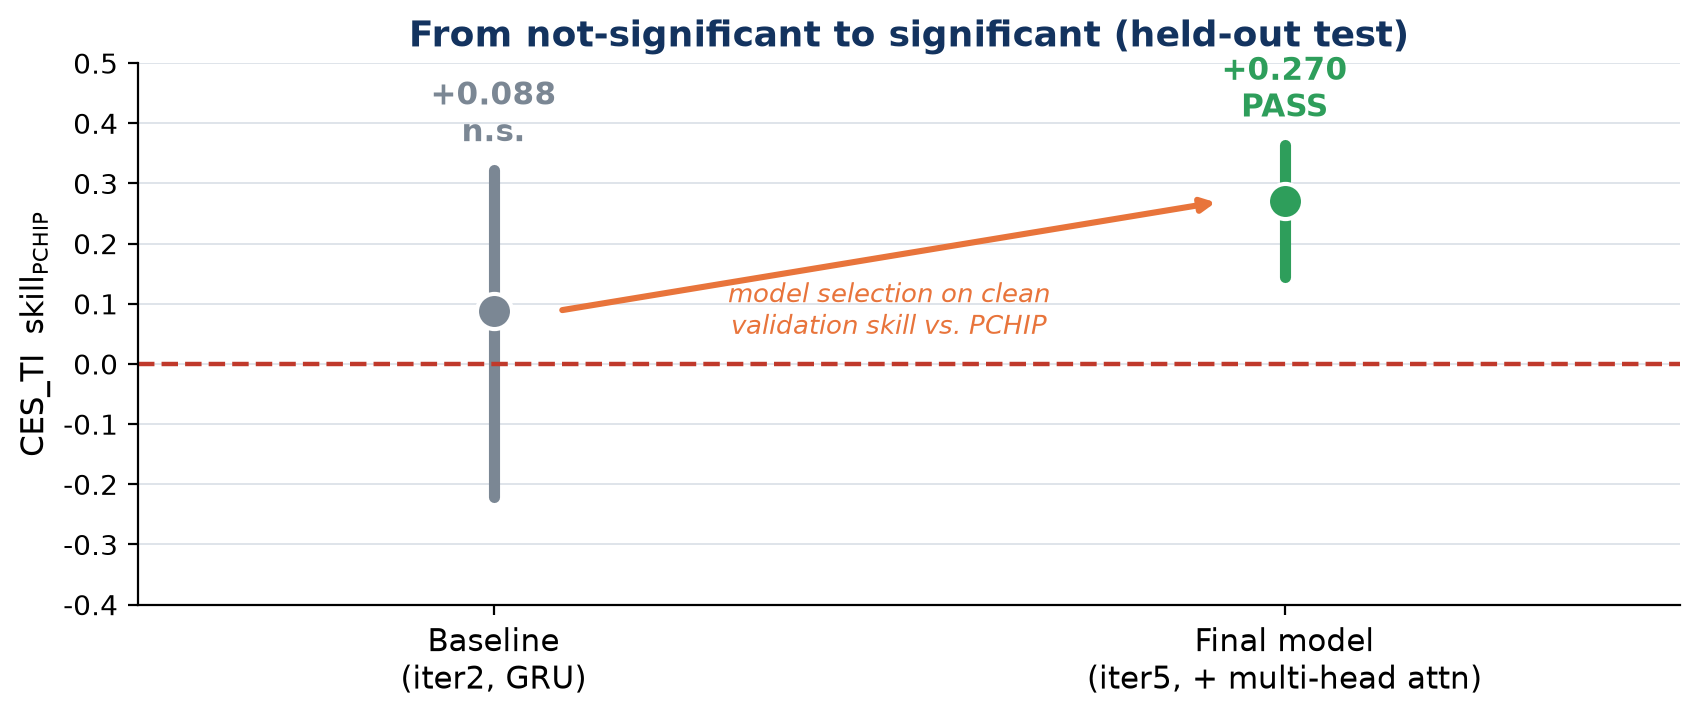
\includegraphics[width=0.7\linewidth]{fig_progression}
  \caption{From non-significant (baseline, $+0.088$ n.s.) to significant
  (final model, $+0.20$--$+0.30$, PASS $\times$4): the decisive change was
  selecting architectures on clean skill rather than validation loss.}
  \label{fig:progression}
\end{figure}

\subsection{Where the skill lives: small gaps dominate}
Stratifying by the time since the last observed CES value, $\geq$97\% of real
targets lie in the small-gap regime ($\Delta t \leq 15$\,ms), where the model wins
(\Ti{} $+0.08$, \Vrot{} $+0.23$ vs.\ PCHIP on the canonical split). At very large
gaps ($>$105\,ms) the future-anchored interpolant dominates, but those bins hold
only tens of samples and carry no per-bin CIs; they are not load-bearing. The one
well-powered comparison---small gaps, which is precisely where nowcasting is
needed---favors the model.

\subsection{The \Ti$\leftrightarrow$\Vrot{} information asymmetry}
\label{sec:asym}
A controlled input-modality ablation (identical training budget; one modality
group zeroed at a time; persistence always computed from real history) explains
\emph{why} the two targets behave differently
(Table~\ref{tab:ablation}, Fig.~\ref{fig:ablation}).

\begin{table}[t]
  \centering
  \caption{Input-modality ablation (validation split, skill vs.\ persistence,
  physical units). Fast diagnostics alone carry genuine \Ti{} information but are
  catastrophically uninformative for \Vrot{}.}
  \label{tab:ablation}
  \small
  \begin{tabular}{lrr}
    \toprule
    Model inputs & \Ti{} skill & \Vrot{} skill \\
    \midrule
    Full (history + fast + time) & $+0.36$ & $+0.18$ \\
    History only (\emph{no fast}) & $+0.39$ & $+0.23$ \\
    Fast diagnostics only (\emph{no history}) & $+0.16$ & $-3.31$ \\
    \bottomrule
  \end{tabular}
\end{table}

\begin{figure}[t]
  \centering
  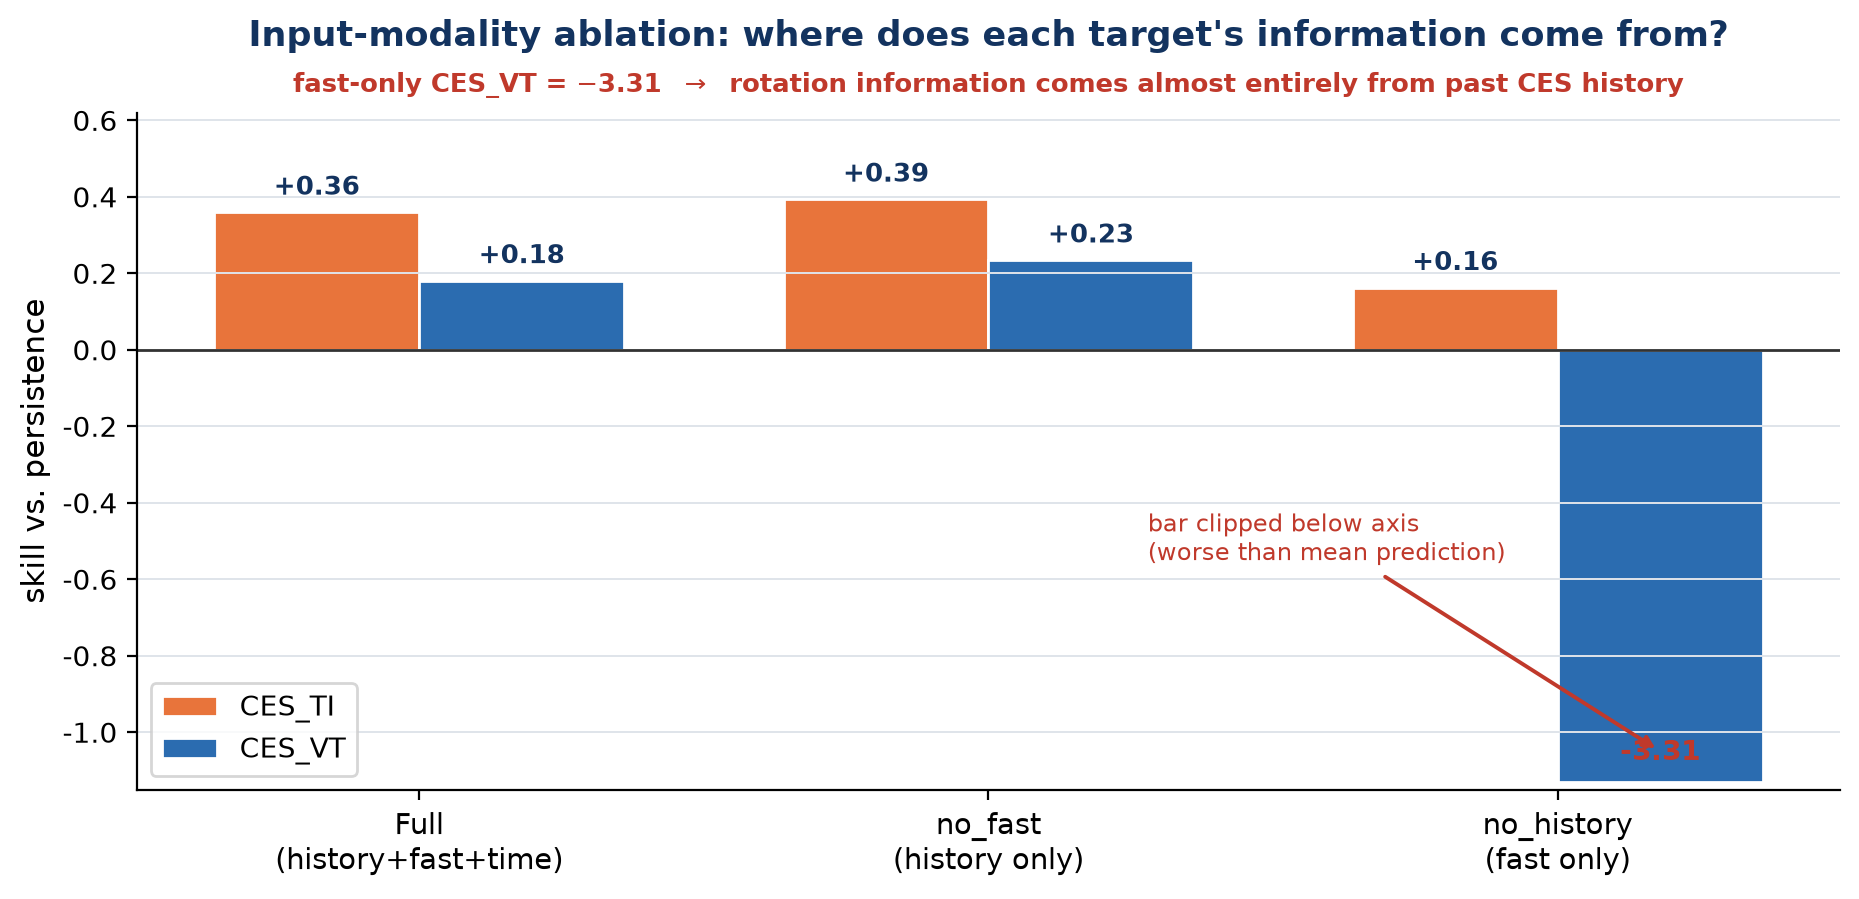
\includegraphics[width=0.75\linewidth]{fig_ablation}
  \caption{Modality ablation: fast-only beats persistence for \Ti{} but is far
  worse than the mean for \Vrot{} --- the information asymmetry.}
  \label{fig:ablation}
\end{figure}

\begin{itemize}
  \item \textbf{\Ti{}: fast diagnostics carry real information.} Fast-only still
        beats persistence ($+0.16$). The physical channel is collisional
        electron--ion coupling ($t_{ei}\propto T_e^{3/2}/n_e$): ECEI supplies
        $T_e$ and BES supplies $n_e$ structure.
  \item \textbf{\Vrot{}: information is almost entirely CES history.} Fast-only
        scores $-3.31$ (worse than predicting the mean). Toroidal rotation is
        governed by momentum sources that none of our inputs observe---the
        external NBI torque and intrinsic rotation
        drives~\citep{Rice2007IntermachineComparison}---and the Mirnov signals are
        sampled at 100\,Hz, aliasing away the kHz mode-rotation frequencies that
        could otherwise proxy rotation.
\end{itemize}

This asymmetry was predicted from physics before the ablation and is confirmed by
it; the \Vrot{} non-win is a finding about diagnostic information content, not a
model failure. It also motivates the per-target routing of \S\ref{sec:model}.

\subsection{The edge concentrates in high-variability neighborhoods}
\label{sec:peak}
Using a target-independent, input-side proxy for local activity (large
neighbor-bracket slope and/or high local CES-neighbor variance, computed
\emph{excluding} the target row), we split evaluation into ``peak''
(high-local-activity) and bulk regions (validation split, shot-clustered CIs;
Fig.~\ref{fig:peak}):

\begin{itemize}
  \item \Ti{}: global $+0.52$ $\rightarrow$ peak $\mathbf{+0.86}$
        (CI $[+0.66, +0.93]$, PASS). Interpolation is near-optimal on the smooth
        bulk; the model's value is in the active stretches.
  \item \Vrot{}: global $+0.24$ $\rightarrow$ peak $\mathbf{+0.69}$
        (CI $[+0.11, +0.87]$, PASS, robust across three sensitivity settings but
        with a thin lower bound). The asymmetry is therefore \emph{regional}:
        globally \Vrot{} ties interpolation, but in high-activity neighborhoods
        --- where smooth past+future interpolation is worst --- even the
        history-driven \Vrot{} predictor adds value. We report this as a regional
        strength on the optimism-caveated validation split, not a reversal of the
        global null result.
  \item A peak-restricted ablation (zeroing BES/ECEI/MC) hurts \Ti{}
        significantly (paired-difference CI $\gg 0$) but leaves \Vrot{} unchanged:
        the \Ti{} peak edge genuinely uses the multimodal signal, while the
        \Vrot{} peak edge is history-driven.
\end{itemize}

\begin{figure}[t]
  \centering
  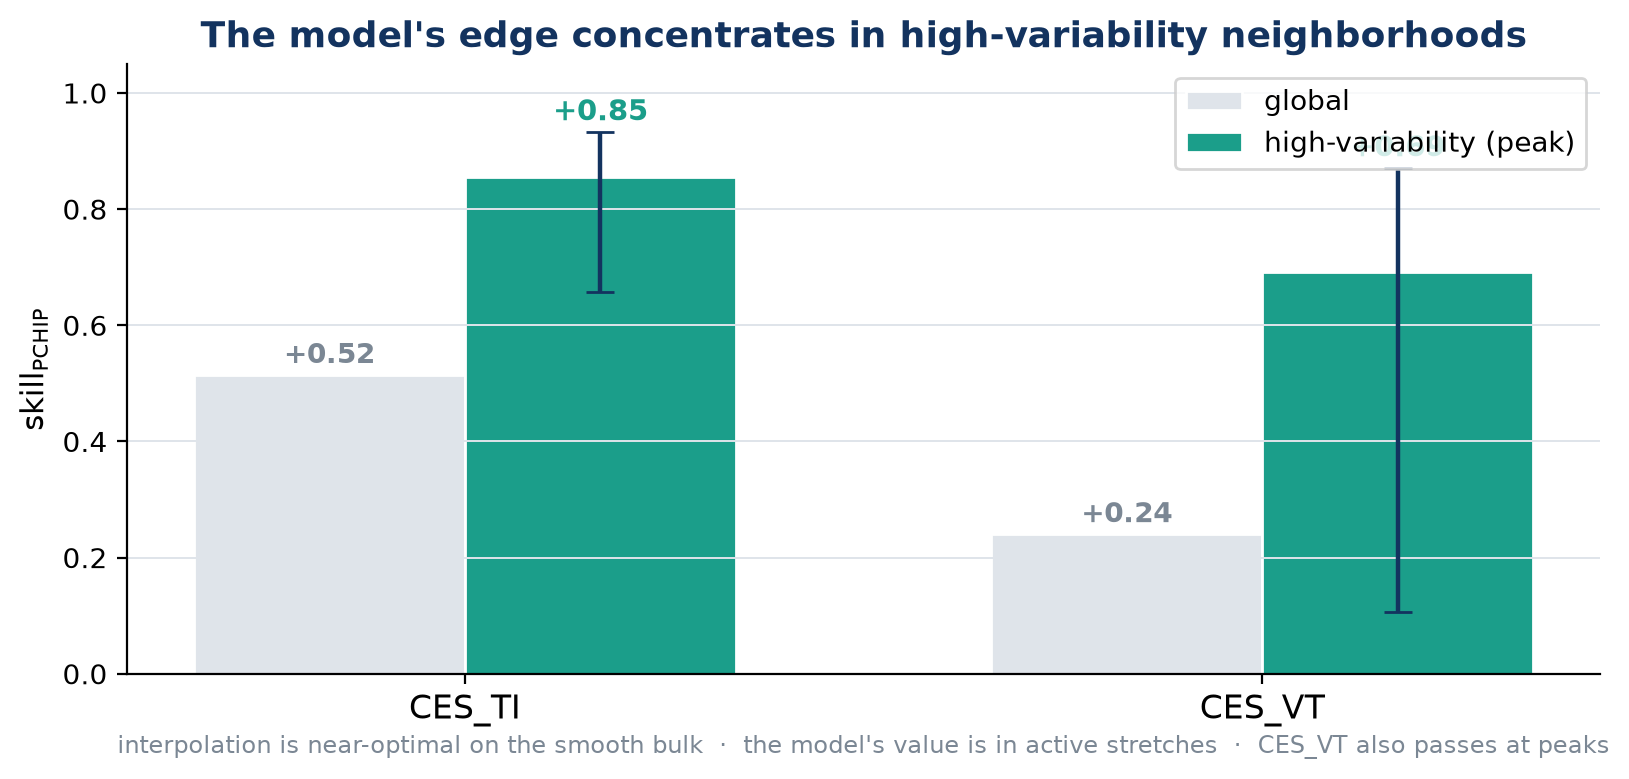
\includegraphics[width=0.78\linewidth]{fig_peak}
  \caption{Global vs.\ high-variability (``peak'') skill with shot-clustered 95\%
  CIs. The model's advantage over interpolation concentrates where interpolation
  is weakest; \Vrot{} passes at peaks despite the global tie.}
  \label{fig:peak}
\end{figure}

% =========================================================================
\section{Search method: an LLM-driven keep/discard loop}
\label{sec:automl}

The final architecture was found by an automated research loop in which an LLM
plays the researcher role (inspired by autoresearch-style keep/discard
protocols). Each iteration: (i) smoke-validate and fully train the current
proposal; (ii) score it on the \emph{clean, non-augmented} validation
$\skillp$---never the augmented validation loss, and never any test split;
(iii) \textbf{keep} the change iff it improves the best score so far, else
\textbf{discard and roll back} \texttt{model.py} to the best snapshot; (iv) brief
the LLM with the run history, a hard data contract (interfaces, masking, and
leakage rules the proposal must preserve), and accumulated project knowledge, and
request \emph{one controlled change}. The loop therefore never builds on a
regression, and training failures are treated as repair signals rather than
evidence. Its concrete contribution here was the n.s.$\to$significant progression
of Fig.~\ref{fig:progression}; we document it as reproducibility infrastructure,
not as the scientific contribution.

% =========================================================================
\section{Limitations}
\label{sec:limits}

\textbf{Statistical power.} The unit of replication is the shot; with
$\approx$96 (\Ti) / 91 (\Vrot) test shots, power bounds every significance call,
and per-shot squared-error differences are heavy-tailed (a few discharges
dominate the bootstrap spread).
\textbf{MNAR optimism.} Skill is measured on observed points only; genuinely
missing points may be harder.
\textbf{Metric asymmetry.} Interpolants use full-shot neighbors while the model
sees a $W{=}4$ history; this is deliberately adverse to the model but complicates
direct interpretation.
\textbf{Single architecture and window.} Sensitivity to $W$ and architecture is
uncharacterized; results are for one selected model.
\textbf{Large-gap bins} contain tens of samples without CIs and are unreliable.
\textbf{Scope.} The pedestal-top framing is inherited from the data selection
(pedestal-top CES channels); no radial-dependence experiment is performed, and
event-phase analyses (ELM cycle, L--H transitions) are future work---the
high-variability analysis of \S\ref{sec:peak} is an event-agnostic proxy.

% =========================================================================
\section{Conclusion}
\label{sec:conclusion}

We built a causal, leakage-hardened multimodal nowcaster for sparse KSTAR CES
targets and evaluated it under a pre-registered, shot-clustered protocol against
a deliberately adverse bar: interpolation that sees the future. The model
decisively beats every causal baseline; for ion temperature it also beats
future-using PCHIP interpolation with significant, replicated skill
($+0.20$--$+0.30$; four independent splits), while toroidal rotation ties
interpolation for a physically identified reason---fast diagnostics simply do not
carry rotation information at 10\,ms. The advantage concentrates exactly where
gap-filling matters: small gaps and high-variability neighborhoods. Beyond the
headline, the work contributes a corrected \Vrot{} evaluation (54\% instrument
holds), an information-asymmetry ablation, and an LLM-driven keep/discard search
protocol. Future work targets the power limitation (more test shots,
multi-campaign data), bracket-distance stratification to isolate the regime where
fast-diagnostic information has maximal marginal value, peak-weighted training,
and rotation-side improvements that better exploit history---since more sensors,
demonstrably, will not help \Vrot{} at this timescale.

% =========================================================================
\subsubsection*{Reproducibility}
Splits are pinned to disk and verified on reload; normalization statistics are
train-file-only; the search loop never reads test data; bootstrap uses a fixed
seed and 10{,}000 resamples; all headline numbers are read from frozen evaluation
artifacts. Code and evaluation artifacts accompany the submission; the public
repository link will be inserted at camera-ready.
% TODO(user): insert repository/DOI link here before submission

\bibliographystyle{unsrtnat}
\bibliography{refs}

\end{document}
